\documentclass[a4paper,10pt,notitlepage]{scrartcl}

\usepackage[T1]{fontenc}
\usepackage[english]{babel}
\usepackage[utf8x]{inputenc}
\usepackage{setspace}
\usepackage{subfig}
\usepackage{textcomp}
\usepackage{graphicx}
\usepackage{fixltx2e}
\usepackage{multirow}
\usepackage{array}
\usepackage{amssymb}
\usepackage{amsmath}
\usepackage{subfig}
\usepackage{nomencl}
\usepackage[pdfborder={0 0 0}]{hyperref}
\usepackage{natbib}
% \usepackage{makeidx}
\usepackage{nicefrac}
\usepackage{bbold}

\captionsetup{labelfont=footnotesize,textfont=footnotesize}

\newcolumntype{x}[1]{>{\begin{flushleft}$}p{#1}<{$\end{flushleft}}}
\newcolumntype{y}[1]{>{\begin{center}$}p{#1}<{$\end{center}}}
\newcolumntype{z}[1]{>{\begin{flushright}$}p{#1}<{$\end{flushright}}}
\newcolumntype{m}{>{$}l<{$}}
\newcolumntype{n}{>{$}c<{$}}
\newcolumntype{o}{>{$}r<{$}}

\newcommand{\mat}[1]{\mathbf{#1}} 

\bibliographystyle{plain}

% Title Page
\title{Scientific Visualization\\Project III}
\author{Milian Wolff}

\begin{document}
\maketitle

\begin{abstract}
During the third project for the the scientific visualization class by Eugene
Zhang we got an introduction to vector calculus and vector field design. We
investigate the topology of vector fields and write a JavaView based
application for LIC-based vector field design and visualization.

The source code of my exercise solutions can be found online under

\begin{center}\url{https://github.com/milianw/scivi}\end{center}
\end{abstract}

\begingroup
\let\clearpage\relax

\tableofcontents
\endgroup

\section{Scalar Field Topology}

In the following we analyze the topology of scalar vector fields defined on
the unit sphere in 3D. We leverage the periodic boundary conditions by applying
spherical coordinates with $r = 1$, which yields the following parametrization:

\begin{equation}
 \vec{r} = \left( \begin{array}{c} x \\ y \\ z \end{array} \right)
        = \left( \begin{array}{c} \cos \phi \sin \theta \\ \sin \phi \sin
\theta \\ \cos \theta \end{array} \right)
\end{equation}

The value ranges are $0 \leq \theta \leq \pi$ and
$0 \leq \phi \leq 2 \pi$.

In the following we investigate scalar vector fields $f(\vec{r})$ and want to
know whether they are Morse, i.e. smooth and have only isolated
and non-degenerate critical points.

The critical points can be found by solving

\begin{equation}
 \nabla f(\vec{r}) = 0,
\end{equation}


with the Nabla-Operator $\nabla$ in spherical coordinates and $r = 1$ being

\begin{equation}
 \nabla = \frac{\partial}{\partial \theta} \vec{e}_\theta + \frac{1}{\sin
\theta} \frac{\partial}{\partial \phi} \vec{e}_\phi.
\end{equation}

Frankly I have no clue how to calculate the Hessian or the determinant
of said in spherical coordinates. I'll thus limit myself to finding the critical
points then.

\subsection{Case a)}

\begin{eqnarray}
 f(\vec{r}) &=& 1 \\
 \nabla f(\vec{r}) &=& 0
\end{eqnarray}

The vector field is not morse since every point is critical and thus
non-isolated.

\subsection{Case b)}

\begin{eqnarray}
 f(\vec{r}) &=& x = \cos\phi \sin\theta \\
 \nabla f(\vec{r}) &=& \cos\phi \cos\theta \vec{e}_\theta - \sin\phi
\vec{e}_\phi
\end{eqnarray}

The above turns zero for $\sin\phi = 0$ and $\cos\theta = 0$, i.e. at $\phi =
0°, 180°$ and $\theta = \pm 90°$. I.e. there are two isolated critical points at
$[\pm 1, 0, 0]^T$.

\subsection{Case c)}

\begin{eqnarray}
 f(\vec{r}) &=& x^2 = \cos^2 \phi \sin^2 \theta \\
 \nabla f(\vec{r}) &=& 2 \cos^2 \phi \cos\theta \sin\theta \vec{e}_\theta -
2 \cos\phi \sin\phi \sin\theta \vec{e}_\phi
\end{eqnarray}

The above turns zero for $\cos\phi = 0$ and any value of $\theta$. As such the
critical points are not isolated and the function non-morse.

\subsection{Case d)}

\begin{eqnarray}
 f(\vec{r}) &=& x^2 - y^2 = \sin^2 \theta( \cos^2 \phi  - \sin^2 \phi) \\
 \nabla f(\vec{r}) &=& 2 \sin \theta \cos \theta (\cos^2 \phi - \sin^2 \phi)
\vec{e}_\theta -
4 \sin \theta \cos\phi \sin\phi \vec{e}_\phi
\end{eqnarray}

The above turns zero for $\sin\theta = 0$, i.e. at the north and
southpole ($\theta = 0, \pi$). It is furthermore zero when $\cos \theta = 0$,
i.e. on the equator, and additionally $\sin \phi = 0$ or $\cos \phi = 0$, i.e.
at $x = \pm 1$ and $y = 0$ or $x = 0$ and $y = \pm 1$.

These singularities are isolated.

\subsection{Case e)}

\begin{eqnarray}
 f(\vec{r}) &=& \sum^N_{k = 0} { \left(\begin{array}{c} N \\ K \end{array}
\right) x^k y^{N-k} \cos \left(\frac{N-k}{2} \pi\right) } \\
  &=& \sin^N \theta \sum^N_{k = 0} { \left(\begin{array}{c} N \\ K \end{array}
\right) \cos^{k}\phi \sin^{N-k} \phi \cos \left(\frac{N-k}{2} \pi\right) } \\
 \nabla f(\vec{r}) &=& \sum^N_{k = 0} { \left(\begin{array}{c} N \\ K
\end{array} \right) \dots }
\end{eqnarray}

For $N = 0$ we have case a), $N = 1$ yields case b). Anything larger boggles my
mind. Lets skip this.

\subsection{Case f)}

\begin{eqnarray}
 f(\vec{r}) &=& x^4 + y^4 + z^4 = \sin^4 \theta ( \cos^4 \phi + \sin^4 \phi ) +
\cos^4 \theta \\
 \nabla f(\vec{r}) &=& 4 (\sin^3 \theta \cos \theta ( \cos^4 \phi + \sin^4 \phi
) - \cos^3 \theta \sin \theta)) \vec{e}_\theta \\
  && + 4 \sin^3 \theta ( \sin^3
\phi \cos \phi - \cos^3 \phi \sin \phi ) \vec{e}_\phi
\end{eqnarray}

There are two critical points once again at $\sin \theta = 0$. For $\cos \theta
= 0$, i.e. on the equator, are again four more singularities for $\cos \phi =
0$ and $\sin \phi = 0$, just like in case d).

\section{Vector Field Design}

The vector field design application is based on JavaView which already has
built-in LIC visualization support. As such, this task was quite easy.

In my implementation, the user picks a type of design element (see below) he
wants to add to the vector field. Then he can add such a feature to the vector
field by clicking into the vector field domain. Existing features can be
removed, altered and moved via drag'n'drop. The view gets updated automatically.

\subsection{Design Elements}

I have decided to implement the following design elements based on the
equations given in the recitation:

\begin{enumerate}
 \item constant, fig \ref{fig:constant}: $\vec{V}_i(\vec{r}) = \sigma
\vec{e}_i$, with $\vec{e}_i$ being a normalized direction vector
 \item generic, fig \ref{fig:generic}: $\vec{V}_i(\vec{r}) = \sigma \mat{A}
(\vec{r} - \vec{r}_i) $, with $\mat{A}$ being an arbitrary $2\times2$~matrix
 \item sink, fig. \ref{fig:sink}: generic with diagonal $\mat{A}$ and entries
$-1$
 \item source, fig \ref{fig:source}: generic with diagonal $\mat{A}$ and
entries $1$
 \item saddle, fig \ref{fig:saddle}: generic with diagonal $\mat{A}$ and
entries $1$ and $-1$
 \item focus, fig \ref{fig:focus}: generic with $\mat{A} = \left(
\begin{array}{cc}
\cos(\theta) & -\sin(\theta) \\
\sin(\theta) & \cos(\theta) \end{array} \right)$
 \item center, clockwise, fig \ref{fig:center-cw}: generic with $\mat{A} =
\left(
\begin{array}{cc}
0 & 1 \\
-1 & 0 \end{array} \right)$
 \item center, counter-clockwise, fig \ref{fig:center-cc}: generic with $\mat{A}
= \left(
\begin{array}{cc}
0 & -1 \\
1 & 0 \end{array} \right)$
 \item converging, fig \ref{fig:converging}: $\sigma (\vec{e}_i + ((\vec{r} -
\vec{r}_i) \cdot \vec{n}_i) \vec{n}_i$, with $\vec{e}_i$ being a normalized
direction vector and $\vec{n}_i$ the normal to that
 \item diverging, fig \ref{fig:diverging}: like the converging element
multiplied by $-1$
\end{enumerate}

In the equations above, $\sigma$ is the scaling factor

\begin{equation}
 \sigma = s \exp(-d |\vec{r}_i - \vec{r}|^2),
\end{equation}

with $s$ denoting the strength and $\vec{r}_i$ being the base point of the
design element, i.e. the point where the user clicked.

Note that user-placed vector field elements are shown as large dots in the LIC
image. They are furthermore color coded such that centers, focuses and sources
and diverging elements are green, while converging elements and sinks are red.
Lastly saddles are colored blue while generic items are black.

\begin{figure}
  \centering
  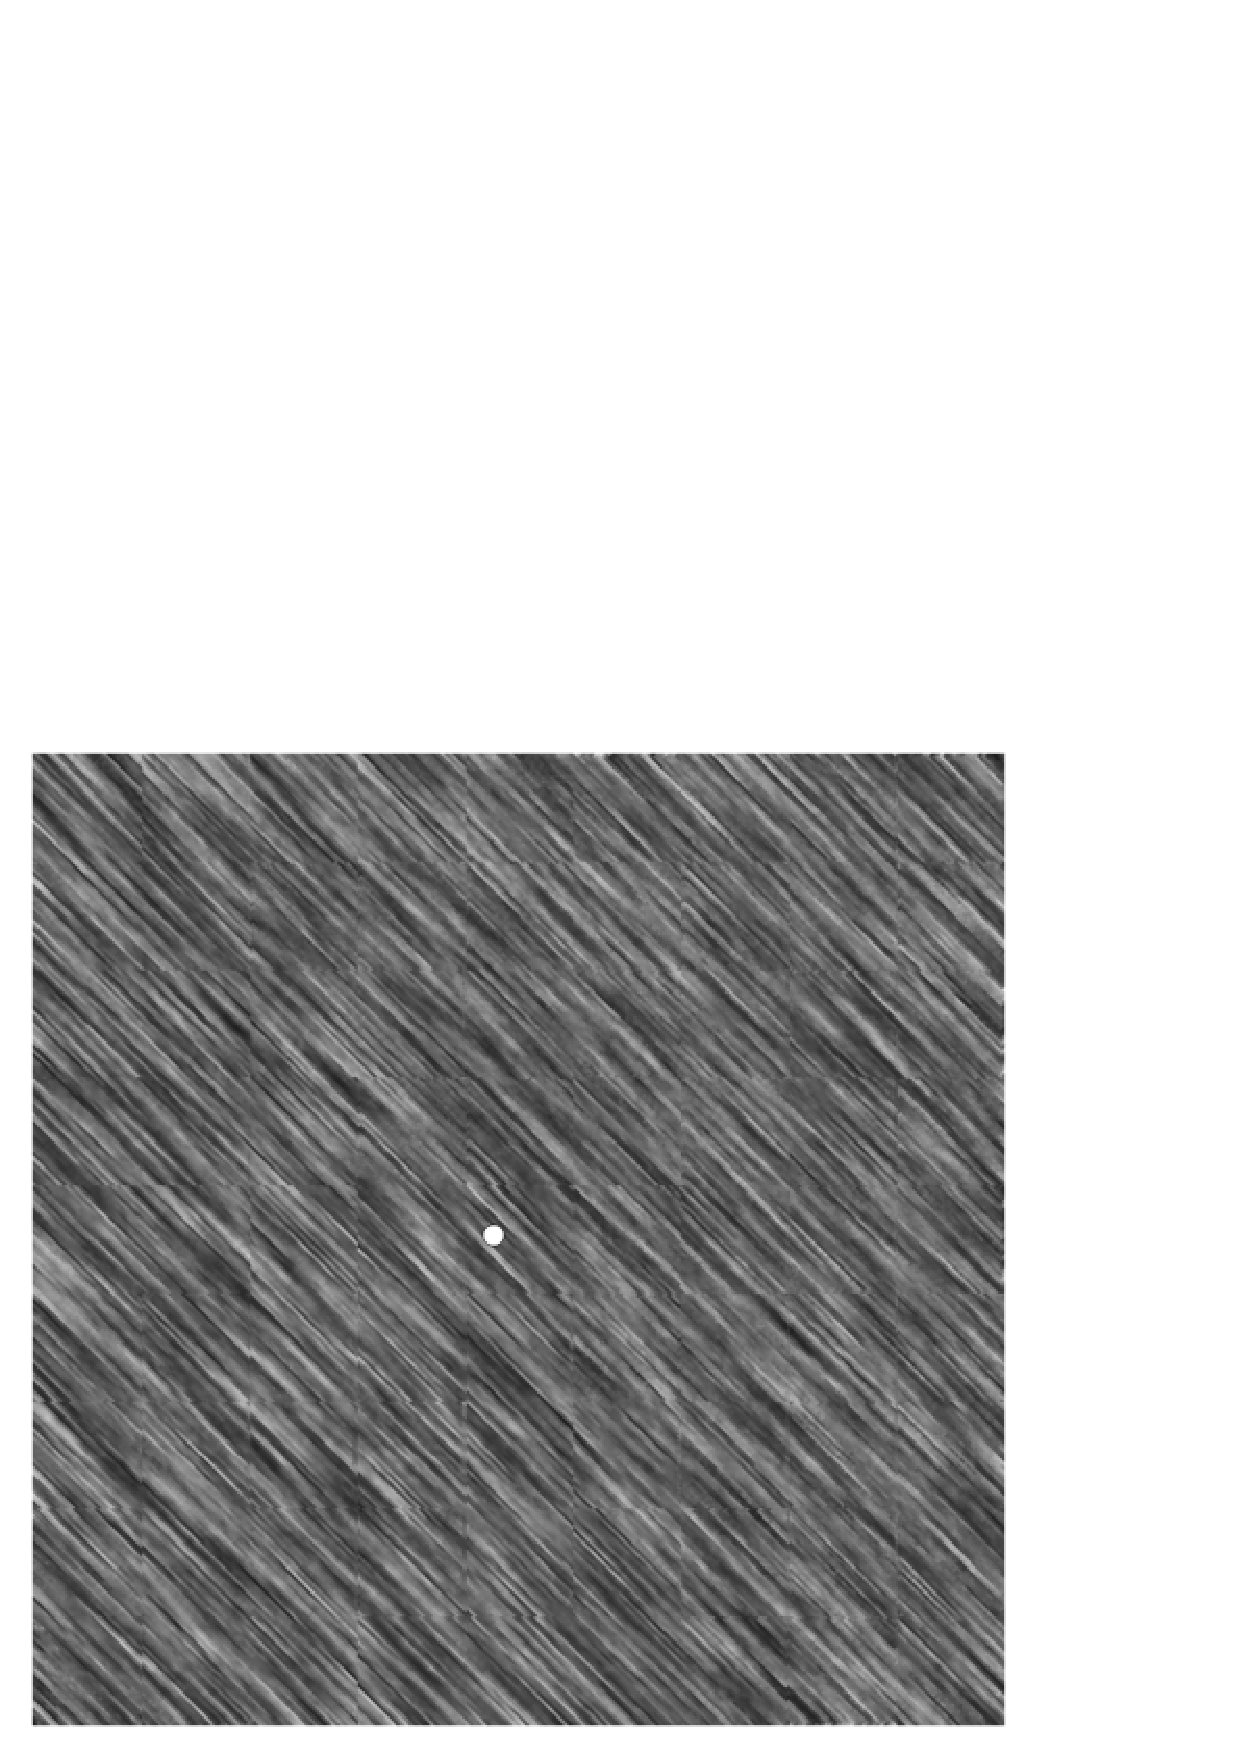
\includegraphics[scale=0.5]{img-3-2/constant.png}
  \caption{constant vector field design element, without decay}
  \label{fig:constant}
\end{figure}

\begin{figure}
  \centering
  \includegraphics[scale=0.5]{img-3-2/generic.png}
  \caption{generic vector field design element}
  \label{fig:generic}
\end{figure}

\begin{figure}
  \centering
  \includegraphics[scale=0.5]{img-3-2/sink.png}
  \caption{sink vector field design element}
  \label{fig:sink}
\end{figure}

\begin{figure}
  \centering
  \includegraphics[scale=0.5]{img-3-2/source.png}
  \caption{source vector field design element}
  \label{fig:source}
\end{figure}

\begin{figure}
  \centering
  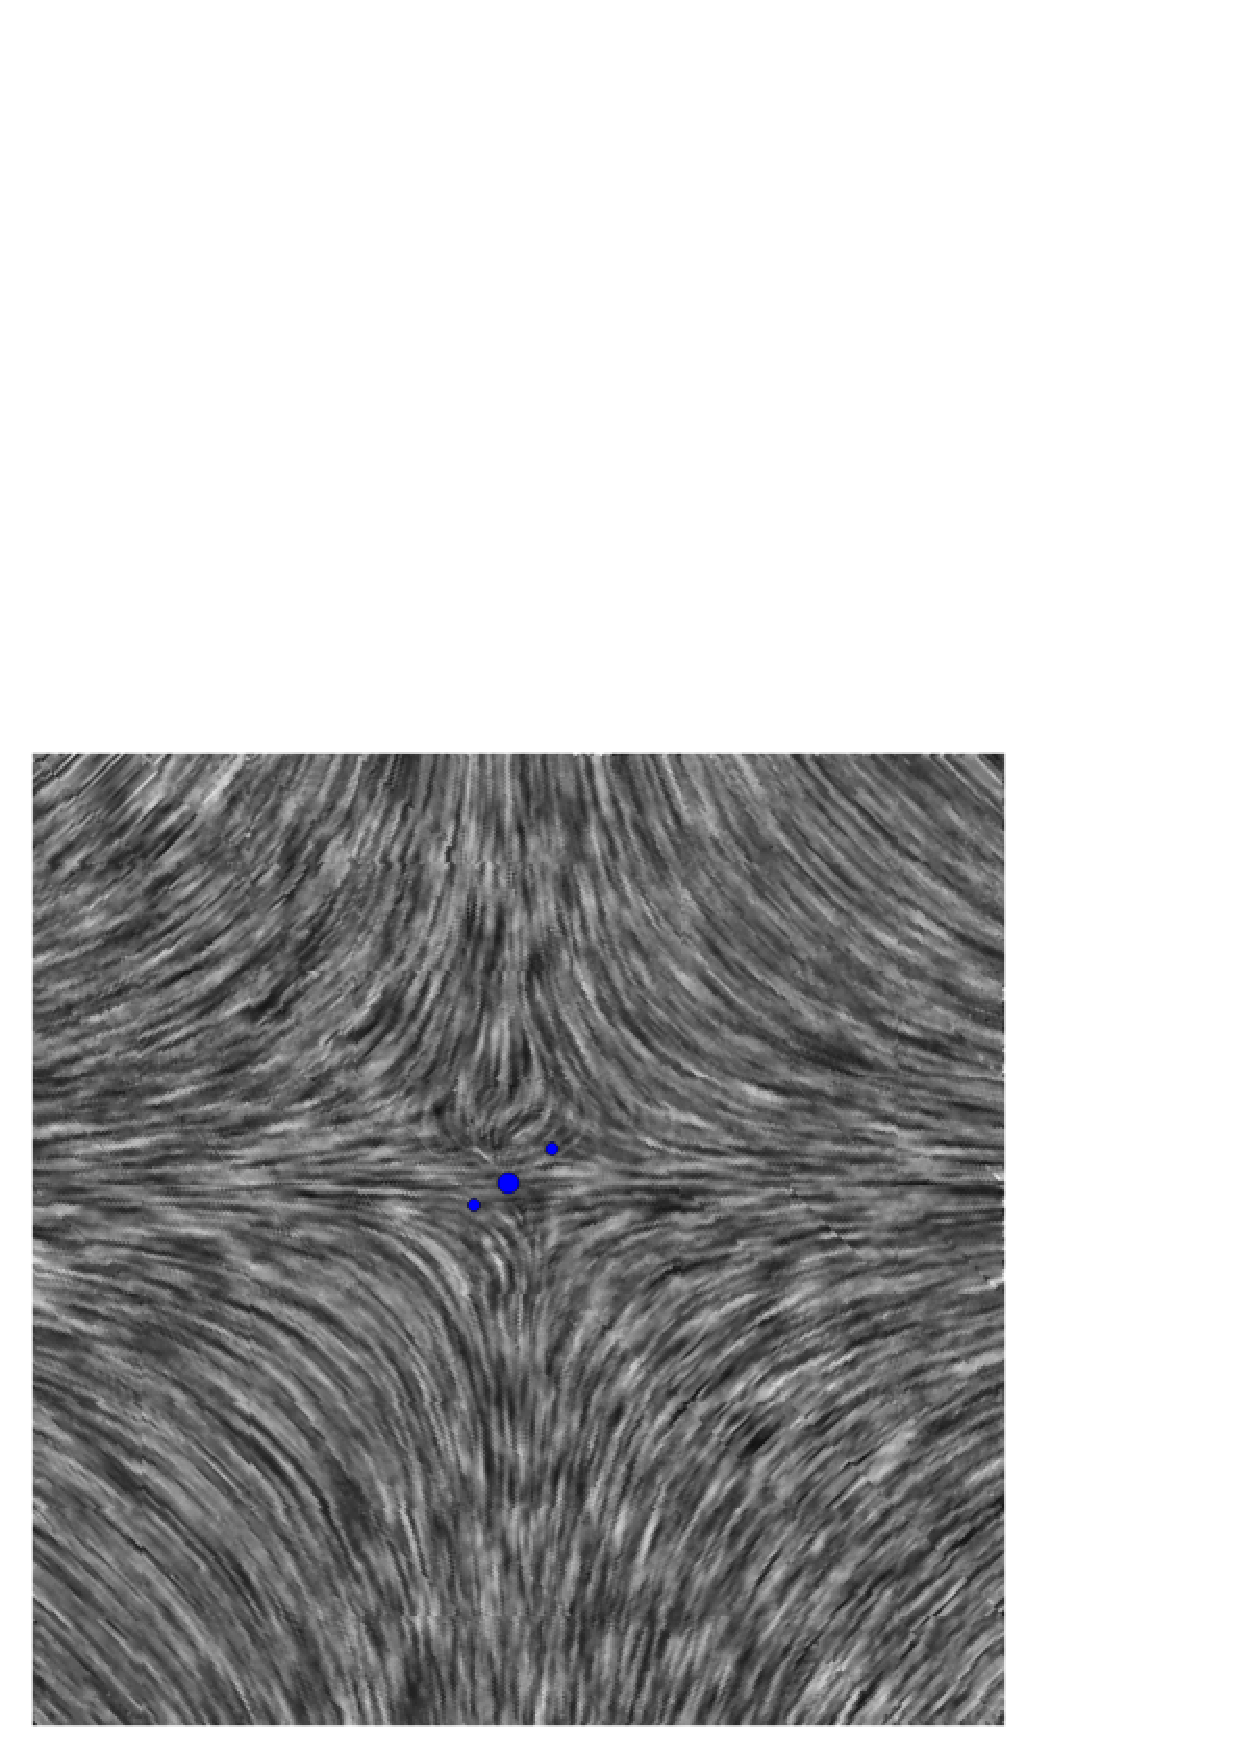
\includegraphics[scale=0.5]{img-3-2/saddle.png}
  \caption{saddle vector field design element}
  \label{fig:saddle}
\end{figure}

\begin{figure}
  \centering
  \includegraphics[scale=0.5]{img-3-2/focus.png}
  \caption{focus vector field design element}
  \label{fig:focus}
\end{figure}

\begin{figure}
  \centering
  \includegraphics[scale=0.5]{img-3-2/center-cw.png}
  \caption{clockwise center vector field design element}
  \label{fig:center-cw}
\end{figure}

\begin{figure}
  \centering
  \includegraphics[scale=0.5]{img-3-2/center-cc.png}
  \caption{counter-clockwise center vector field design element}
  \label{fig:center-cc}
\end{figure}

\begin{figure}
  \centering
  \includegraphics[scale=0.5]{img-3-2/converging.png}
  \caption{converging vector field design element}
  \label{fig:converging}
\end{figure}

\begin{figure}
  \centering
  \includegraphics[scale=0.5]{img-3-2/diverging.png}
  \caption{diverging vector field design element}
  \label{fig:diverging}
\end{figure}

\subsection{Parametrization}

I reuse the given parametrization of the plane in a triangulated quad. I have
chosen a equidistant discretization of $10 \times 10 = 100$ vertices. The
discrete vector field is then given by evaluating the sum of all design
elements at each vertex point.

\subsection{Flow Rotation}

The flow can easily rotated by an arbitrary angle $\theta$ via
matrix-multiplication of each vector in the discretized domain with a rotation
matrix:

\begin{equation}
 \vec{v}'(\vec{r}) = \mat{R} \vec{v}(\vec{r})
\end{equation}

The rotation matrix is given by

\begin{equation}
 \mat{R} = \left(
\begin{array}{cc}
\cos(\theta) & -\sin(\theta) \\
\sin(\theta) & \cos(\theta) \end{array} \right)
\end{equation}

An example can be seen in fig. \ref{fig:flow-rotation}.

\begin{figure}
  \centering
  \subfloat[basis]{
    \includegraphics[scale=0.5]{img-3-2/rotate-a.png}}
  \\
  \subfloat[rotated]{
    \includegraphics[scale=0.5]{img-3-2/rotate-b.png}}
  \caption{flow rotation}
  \label{fig:flow-rotation}
\end{figure}

\subsection{Flow Reflection}

Similar to above, flow reflection is achieved via matrix multiplication. In my
implementation, reflection can be turned on and off and is supposed to be used
in combination with flow rotation. When flow reflection is turned on, the sign
of the second column in the rotation matrix changes sign:

\begin{equation}
 \mat{R}' = \mat{R} \cdot \left( \begin{array}{c} 1 \\ -1\end{array} \right)
\end{equation}

An example for flow reflection is shown in fig. \ref{fig:flow-reflection}.

\begin{figure}
  \centering
  \subfloat[basis]{
    \includegraphics[scale=0.5]{img-3-2/reflect-a.png}}
  \\
  \subfloat[reflected]{
    \includegraphics[scale=0.5]{img-3-2/reflect-b.png}}
  \caption{flow reflection}
  \label{fig:flow-reflection}
\end{figure}

\subsection{Singularities}

Whenever the vector field is updated, I extract the singularities while LIC is
running in the background. To do so we first need to interpolate the discretized
vector field, yielding an element-wise continous vector field.

\subsubsection{Vector Field Interpolation}

For each element, i.e. triangle we first combine the three vertex positions
into a matrix

\begin{equation}
 \mat{A} = \left(
\begin{array}{ccc}
x_1 & y_1 & 1 \\
x_2 & y_2 & 1 \\
x_3 & y_3 & 1 \end{array} \right).
\end{equation}

The actual values of the discrete vector field we store in two vectors
$\vec{b}_x$ and $\vec{b}_y$ such that

\begin{equation}
 \vec{b}_{k} = \left( \begin{array}{c} k_1 \\ k_2 \\ k_3 \end{array} \right) .
\qquad k = x,y
\end{equation}

Now we can solve, using the Cramer method, the following two equations:

\begin{equation}
 \mat{A} \vec{c}_k = \vec{b}_k \qquad k = x,y
\end{equation}

We obtain six coefficients which define our interpolated vector field:

\begin{eqnarray}
 \vec{V}'_i(\vec{r}) &=& \left(
\begin{array}{cc}
c_{x,1} & c_{x,2} \\
c_{y,1} & c_{y,2} \end{array} \right) \vec{r} + \left( \begin{array}{c} c_{x,3}
\\ c_{y,3} \end{array} \right) \\
 &=& \mat{C} \vec{r} + \vec{c}
\label{eq:interpolated-field}
\end{eqnarray}

The above is implemented in \texttt{InterpolatedField::interpolate()}.

\subsubsection{Finding Singularities}

Using eq. \ref{eq:interpolated-field} we can easily find singularities by
solving the equation

\begin{equation}
 \mat{C} \vec{r}_s = - \vec{c}.
 \label{eq:singularity}
\end{equation}

One must consider the boundary though, i.e. our interpolated vector field is
only valid inside the triangle area. Hence a solution obtained by
eq. \ref{eq:singularity} is only a ``real'' singularity if $\vec{r}_s$ is
inside the triangle. The latter is easily checked by the usual vector
multiplication approach as implemented in \texttt{::inTriangle()} and
\texttt{::onSameSide()}. All the above is implemented in cmp.
\texttt{::findSingularities()}.

\subsubsection{Classification}

To classify the singularities found by applying the above method, we look at
the eigenvalues of the Jacobian, in our case $\mat{C}$. If the two eigen values
have a different sign, i.e. $\sigma(\lambda_1) \neq \sigma(\lambda_2)$ then the
singularity is a saddle. Otherwise the singularity is a sink if the eigenvalues
are negative and a source otherwise, i.e. for positive eigenvalues.

\subsubsection{Examples}

Two examples of the above algorithm to find singularities can be seen in fig.
\ref{fig:singularities}. The singularities are again color coded similar to
above and can be differentiated from the user-supplied design terms by their
smaller size.

\begin{figure}
  \centering
  \subfloat{
    \includegraphics[scale=0.4]{img-3-2/singularities-a.png}}
  \\
  \subfloat{
    \includegraphics[scale=0.4]{img-3-2/singularities-b.png}}
  \caption{finding singularities}
  \label{fig:singularities}
\end{figure}

\subsection{Separatrices}

After having found the singularities in the vector field we can go one step
further by also visualizing the separatrices, i.e. the two isolines originating
at a saddle and going into the major and minor direction of the Jacobian
$\mat{C}$.

\subsubsection{Line Tracing}

To trace an separatrix we take a seed $\vec{y_0}$ that is slightly displaced
from the singularity in the direction we want to go to. The next point on the
separatrix is then found by numeric integration, e.g. via the explicit Euler
method (cmp. \texttt{ExplicitEulerTracer}):

\begin{equation}
 \vec{y}_{i+1} = \vec{y}_i + h \vec{V}(\vec{y}_i)
\end{equation}

Here $\vec{V}$ denotes the interpolated vector field that is valid at the
position $\vec{y}_i$, see \texttt{InterpolatedField::elementAt()} for more
information.

A better approach is to apply the so called classical Runge-Kutta
metod (cmp. \texttt{ClassicalRungeKuttaTracer}), which is more numerically
stable. Here we obtain the next line node from the equation

\begin{equation}
 \vec{y}_{i+1} = \vec{y}_i + \nicefrac{1}{3} (\vec{k}_1 + 2 \vec{k}_2 + 2
\vec{k}_3 + \vec{k}_4),
\end{equation}

with

\begin{eqnarray}
 \vec{k}_1 &=& h \vec{V}(\vec{y}_i) \\
 \vec{k}_2 &=& h \vec{V}(\vec{y}_i + 0.5 \vec{k}_1) \\
 \vec{k}_3 &=& h \vec{V}(\vec{y}_i + 0.5 \vec{k}_2) \\
 \vec{k}_4 &=& h \vec{V}(\vec{y}_i + \vec{k}_3).
\end{eqnarray}

\subsubsection{Caveats}

There are no built-in checks to prevent crossing separatrices, which may result
in noisy images esp. when multiple saddles are in the vicinity of a vortex.

Furthermore the tracer does not stop when it gets close to a singularity, which
sometimes might lead to a small overshoot, yet most of the time can be safely
ignored.

Both of the above could be implemented but will impose a significant
performance burden.

\subsubsection{Examples}

To see the above in action, look at fig. \ref{fig:separatrices}. Note that
separatrices in major direction are colored cyan while those in the minor
direction are orange. Furthermore each integration step is shown by a vertex
node on the separatrix.

My implementation uses the classical Runge-Kutta integration scheme with a
stepsize of $h = 0.5$ and up to $N = 1000$ steps.

\begin{figure}
  \centering
  \subfloat{
    \includegraphics[scale=0.4]{img-3-2/separatrices-a.png}}
  \\
  \subfloat{
    \includegraphics[scale=0.4]{img-3-2/separatrices-b.png}}
  \caption{finding separatrices}
  \label{fig:separatrices}
\end{figure}

\end{document}

% kate: replace-tabs on;